\documentclass[../main.tex]{subfiles}

\begin{document}
\begin{questions}

\question Consider a planar surface $\mathcal{S}$ parallel to $xy$ plane bounded by a closed curve $\mathcal{C}$. Consider a vector field
\begin{equation*}
	\vec{F} = 0.5(-y\,\ihat + x\,\jhat)
\end{equation*}
Prove that the value of the integral of this vector field along the curve $\mathcal{C}$ is exactly equal to the area of the planar surface $\mathcal{S}$. Using this find the area inside the curve $x^{\frac{2}{3}}+y^{\frac{2}{3}}=1$

\begin{solution}
	We have to prove some line integral to be equal to some area integral. Stokes' theorem immediately springs to mind (this kind of application of Stokes' theorem on a plane is another theorem called Green's theorem).
	\begin{align}
		\oint_\mathcal{C} \vec{F}\cdot d\vec{l} &= \iint_\mathcal{S} \nabla\times\vec{F}\cdot d\hat{n}\\
		&= \iint_\mathcal{S} \khat \cdot dx\,dy\,\khat\\
		&= \iint_\mathcal{S} dx\,dy\\
		&= \text{Area}(S)\\
	\end{align}
	Thus we can use this to find the area enclosed inside any curve. Let $\mathcal{C}$ be the curve defined by $x^{\frac{2}{3}}+y^{\frac{2}{3}}$, and $\mathcal{S}$ be the region enclosed by this curve. Let us parametrize $\mathcal{C}$ using the paremeter $t$
	\begin{align}
		\mathcal{C} &\coloneqq \Set{(\cos^3t,\,\sin^3t)}{0 \leq t < 2\pi}\\
		d\vec{l} &= dx\,\ihat + dy\,\jhat\\
		&= -3\cos^2t\sin t\,\ihat + 3\sin^2t\cos t\,\jhat
	\end{align}
	\begin{align}
		\text{Area}(S) &= \oint_\mathcal{C} \vec{F}\cdot d\vec{l}\\
		&=\frac{1}{2}\int_{t=0}^{2\pi} (-\sin^3t) (-3\cos^2t\sin t) + (\cos^3t)(3\sin^2t\cos t)\,dt\\
		&=\frac{3}{2}\int_{t=0}^{2\pi} \sin^2t\cos^2t\,dt\\
		&=\frac{3}{8}\int_{t=0}^{2\pi} \sin^22t\,dt\\
		&=\frac{3}{16}\int_{t=0}^{4\pi} \sin^2t\,dt\\
		&=\frac{3}{4}\int_{t=0}^{\pi} \sin^2t\,dt\\
		&= \frac{3\pi}{8}
	\end{align}
\end{solution}

\question A ship sails from the southernmost point of India ($6.75^{o}$N, $93.84^{o}$E) to the southernmost point of Africa ($34.5^{o}$S, $20.00^{o}$E) following the shortest possible path.
\begin{parts}
	\part Given that the radius of the earth is $6400$ km, what is the distance it has covered?
	\begin{solution}
		We cannot directly calculate the distance. We need the angle subtended by the path on Earth's centre. For that we need to convert to Cartesian coordinates
		\begin{align}
			\vec{r_1} &= R\sin\theta_1\cos\phi_1\,\hat{\imath} + R\sin\theta_1\sin\phi_1\,\hat{\jmath} + R\cos\theta_1\,\hat{k} = R(-0.067\,\hat{\imath}-0.991\,\hat{\jmath}+0.118\,\hat{k})\\
			\vec{r_2} &= R\sin\theta_2\cos\phi_2\,\hat{\imath} + R\sin\theta_2\sin\phi_2\,\hat{\jmath} + R\cos\theta_2\,\hat{k} = R(0.774\,\hat{\imath}-0.282\,\hat{\jmath}-0.566\,\hat{k})
		\end{align}
		Where,
		\begin{description}
			\item[R] = $6400$ km
			\item[$\theta_1$] = $90^o-6.75^o=83.25^o$
			\item[$\theta_2$] = $90^o+34.5^o=124.5^o$
			\item[$\phi_1$] = $-93.84^o$
			\item[$\phi_2$] = $-20^o$
		\end{description}
		Let $\theta'$ be the angle between $\vec{r_1}$ and $\vec{r_2}$.
		\begin{align}
			\cos\theta' &= \frac{\vec{r_1}\cdot\vec{r_2}}{|\vec{r_1}||\vec{r_2}|} \\
			&= \frac{R^2(-0.067\cdot0.774+0.991\cdot0.282-0.118\cdot0.566)}{R\cdot R} = 0.161 \\
			\implies \theta' &= \cos^{-1}0.161 = 1.409 \text{ rad}
		\end{align}
		Now we can get the distance by $R\,\theta'=6400$ km $ \cdot $ $ 1.409=9017 $ km
	\end{solution}
	\newpage
	\part If instead of sailing, one had travelled in an aeroplane - by what percentage would the shortest possible distance change?
	\begin{solution}
		The change in distance will only be due to the change in $R$, as $R$ will be increased by the cruising altitude of an aeroplane $\approx10$ km. So percentage change $ = $ $\frac{10}{6400}=0.15\%$
	\end{solution}
\end{parts}

\question Compute the divergence of the vector field given by:
\begin{equation*}
	\vec{v} \,=\, r\cos\theta\, \hat{r} ~+~ r\sin\theta\, \hat{\theta} ~+~ r\sin\theta\cos\phi\, \hat{\phi} 
\end{equation*}
Check the divergence theorem for this using the volume of an inverted hemisphere of radius $R$, resting on the $xy$ plane and centered at the origin.
\begin{solution}
	\label{div}
	Let us first calculate the divergence of $\vec{v}$
	\begin{equation}
		\nabla\cdot\vec{v} = \frac{1}{h_rh_\theta h_\phi} \left( \frac{\partial (v_r h_\theta h_\phi)}{\partial r} + \frac{\partial (h_r v_\theta h_\phi)}{\partial \theta} + \frac{\partial (h_r h_\theta v_\phi)}{\partial \phi} \right)
	\end{equation}
	where
	\begin{description}
		\item[$h_r$] = Scale factor of $r = 1$
		\item[$h_\theta$] = Scale factor of $\theta = r$
		\item[$h_\phi$] = Scale factor of $\phi = r\sin\theta$
	\end{description}
	\begin{align}
		\implies \nabla\cdot\vec{v} &= \frac{1}{r^2\sin\theta}\left( \frac{\partial (r^3\sin\theta\cos\theta)}{\partial r} + \frac{\partial (r^2\sin^2\theta)}{\partial \theta} + \frac{\partial (r^2\sin\theta\cos\phi)}{\partial \phi}\right) \\
		&= \frac{1}{r^2\sin\theta}\left( 3r^2\sin\theta\cos\theta + 2r^2\sin\theta\cos\theta - r^2\sin\theta\sin\phi \right) \\
		&= 5\cos\theta - \sin\phi
	\end{align}

	Now we need to check the divergence theorem for the hemisphere
	\begin{center}
		\tdplotsetmaincoords{80}{45}
		\begin{tikzpicture}[tdplot_main_coords]
			\draw[thick,->] (0,0,0) -- (3,0,0) node[anchor=north east]{$x$};
			\draw[thick,->] (0,0,0) -- (0,3,0) node[anchor=north west]{$y$};
			\draw[thick,->] (0,0,0) -- (0,0,3) node[anchor=south]{$z$};

			\draw[tdplot_screen_coords] (1.8,0) arc (0:180:1.8);

			\begin{scope}[canvas is xy plane at z=0]
				\draw (-1.2728,-1.2728) arc (-135:45:1.8);
				\draw[dashed] (1.2728,1.2728) arc (45:225:1.8);
			\end{scope}

			\draw (0,0,1.8) node[anchor=south west]{$R$} node[anchor=south east]{$S_1$};
			\draw (0,0,0) node [yshift=-20]{$S_2$};
		\end{tikzpicture}
	\end{center}

	According to divergence theorem
	\begin{equation}
		\iiint_V \nabla\cdot\vec{v}\,dV = \oiint_S \vec{v}\cdot d\vec{S}
	\end{equation}

	Let us first calculate the LHS. For that we need $dV$. We know that for spherical polar coordinates, $dV = h_r h_\theta h_\phi\,dr\,d\theta\,d\phi = r^2\sin\theta\,dr\,d\theta\,d\phi$

	\begin{align}
		\text{LHS } = \iiint_V \nabla\cdot\vec{v}\,dV &= \int^{\phi=2\pi}_{\phi=0}\int^{\theta=\frac{\pi}{2}}_{\phi=0}\int^{r=R}_{r=0} (5\cos\theta-\sin\phi) \,r^2\sin\theta\,dr\,d\theta\,d\phi \\
		&= \frac{R^3}{3}\int^{\phi=2\pi}_{\phi=0}\int^{\theta=\frac{\pi}{2}}_{\theta=0} (5\sin\theta\cos\theta - \sin\theta\sin\phi)\, d\theta\,d\phi \\
		&= \frac{5\pi R^3}{3}
	\end{align}

	For the RHS we need $d\vec{S}$. But the surface has 2 parts, the hemispherical cap $S_1$ and the base $S_2$. Now for spherical coordinates you know that $d\vec{S_1} = d\vec{S_r} = h_\theta h_\phi \,d\theta\, d\phi\, \hat{r} = r^2\sin\theta\, d\theta\, d\phi\, \hat{r}$. You can also find this using parametrization. We can see (using visualization or parametrization) that $d\vec{S_2} = r\,dr\,d\phi\,\hat{\theta}$.

	\begin{align}
		\eval{\vec{v}}_{S_1} = \eval{\vec{v}}_{r=R} &= R\cos\theta\,\hat{r} + R\sin\theta\,\hat{\theta} + R\sin\theta\cos\phi\,\hat{\phi} \\
		\eval{\vec{v}}_{S_2} = \eval{\vec{v}}_{\theta=\frac{\pi}{2}} &= r\,\hat{\theta} + r\cos\phi\,\hat{\phi}
	\end{align}
	\begin{align}
		\implies \text{RHS } = \oiint_{S_1} \vec{v}\cdot d\vec{S_1} + \oiint_{S_2} \vec{v}\cdot d\vec{S_2}  &= \int^{\phi=2\pi}_{\phi=0}\int^{\theta=\frac{\pi}{2}}_{\theta=0} (R\cos\theta)\,R^2\sin\theta\,d\theta\,d\phi \\
		&+ \int^{\phi=2\pi}_{\phi=0}\int^{r=R}_{r=0} (r)\,r\,dr\,d\theta\\
		&= \int^{\phi=2\pi}_{\phi=0}\int^{\theta=\frac{\pi}{2}}_{\theta=0} R^3\sin\theta\cos\theta\,d\theta\,d\phi \\
		&+ \int^{\phi=2\pi}_{\phi=0}\int^{r=R}_{r=0} r^2\,dr\,d\theta \\
		&= \pi R^3 + \frac{2\pi R^3}{3} = \frac{5\pi R^3}{3} = \text{ LHS} \hskip0.15\textwidth\blacksquare
	\end{align}
\end{solution}

\question Compute the line integral of $\vec{F} = (2xz + y, 2yz + 3x, x^2 + y^2 + 5)$. Use Stokes’ theorem to compute \[\oint\limits_{\mathcal{C}} \vec{F}\cdot \vec{\mathrm{d}r}\] $\mathcal{C}$ is any positively oriented curve on the surface of the circular cylinder of radius 1 with it's axis along the +ve $y$ axis and with one face as the $xy$ plane with O as centre. 
\begin{solution}
	\begin{center}
		\tdplotsetmaincoords{80}{45}
		\begin{tikzpicture}[tdplot_main_coords]
			\draw[thick,->] (0,0,0) -- (3,0,0) node[anchor=north west]{$x$};
			\draw[thick,->] (0,0,0) -- (0,3,0) node[anchor=south west]{$y$};
			\draw[thick,->] (0,0,0) -- (0,0,3) node[anchor=south]{$z$};

			\begin{scope}[canvas is xy plane at z=0]
				\draw[very thick] (0,0) circle (1.5);
			\end{scope}
			\begin{scope}[canvas is xy plane at z=2]
				\draw (0,0) circle (1.5);
			\end{scope}

			\draw ({1.5*sqrt(0.5)},{1.5*sqrt(0.5)},0) -- ({1.5*sqrt(0.5)},{1.5*sqrt(0.5)},2);
			\draw ({-1.5*sqrt(0.5)},{-1.5*sqrt(0.5)},0) node[anchor=north]{$\mathcal{C}_1$} -- ({-1.5*sqrt(0.5)},{-1.5*sqrt(0.5)},2);

			\begin{scope}[canvas is plane={O(0,0,1)x(1,0,1.1)y(0,1,1.1)}]
				\draw[very thick] (0,0) circle (1.5);
			\end{scope}

			\draw ({-1.5*sqrt(0.5)},{-1.5*sqrt(0.5)},0.8) node[anchor=east]{$\mathcal{C}$};

			\draw (0,0,0.5) node[anchor=west]{$\mathcal{S}$};

		\end{tikzpicture}
	\end{center}

	Let $\mathcal{C}_1$ be the unit circle on the $z=0$ plane with the same orientation as $\mathcal{C}$ and $\mathcal{S}$ is the surface on the cylinder enclosed between $\mathcal{C}$ and $\mathcal{C}_1$, with the normal direction such that it matches the orientation of $\mathcal{C}$\\
	Now, by Stokes theorem
	\begin{align}
		-\oint_{\mathcal{C}_1}\vec{F}\cdot d\vec{l} + \oint_{\mathcal{C}}\vec{F}\cdot d\vec{l} &= \iint_\mathcal{S} \nabla\times\vec{F}\cdot d\hat{n}
\intertext{But,}
		\nabla\times\vec{F} &= 2\,\khat\\
		\implies \iint_\mathcal{S} \nabla\times\vec{F}\cdot d\hat{n} &= 0
\intertext{Since $d\hat{n}\cdot \khat = 0$}
		\implies \oint_{\mathcal{C}}\vec{F}\cdot d\vec{l} &= \oint_{\mathcal{C}_1}\vec{F}\cdot d\vec{l}
	\end{align}
	Thus the line integral of any closed curve on the cylinder (which goes around the cylinder) is equal to the line integral of the unit circle at $z=0$ plane centered at origin. Let us find this line integral\\
	Paremetrizing $\mathcal{C}_1$ using the variable $t$
	\begin{align}
		\mathcal{C}_1 &\coloneqq \Set{(\cos t, \sin t, 0)}{0\leq t < 2\pi}\\
		\implies d\vec{l} &= dx\,\ihat + dy\,\jhat\\
		&= -\sin t\,\ihat+\cos t\,\jhat\\
		\implies \oint_{\mathcal{C}_1}\vec{F}\cdot d\vec{l} &= \int_{t=0}^{2\pi} (\sin t)(-\sin t) + (3\cos t)(\cos t)\,dt\\
		&= \boxed{2\pi}
	\end{align}
\end{solution}

\question  If $\vec{a}$ and $\vec{b}$ are constant vectors, $\phi (\vec{r}) = (\vec{a} \times \vec{r}) \cdot (\vec{b} \times \vec{r}) $ is the potential over all space, then find the electric field and charge density in spherical co-ordinates.
\newline
[Hint: $\vec{E} = -\nabla\phi$, $\rho = \epsilon_0 \nabla\cdot \vec{E}$]
\begin{solution}
	First let us simplify $\phi(\vec{r})$
	\begin{align}
		\phi (\vec{r}) &= (\vec{a} \times \vec{r}) \cdot (\vec{b} \times \vec{r})\\
		&= \vec{a}\cdot (\vec{r} \times \vec{b} \times \vec{r}) && \text{$\because$ $\vec{a}\times\vec{b}\cdot\vec{c}=\vec{a}\cdot\vec{b}\times\vec{c}$}\\
		&= \vec{a}\cdot((\vec{r}\cdot\vec{r})\vec{b}-(\vec{b}\cdot\vec{r})\vec{r}) && \text{The \textit{bac-cab} rule}\\
		&= r^2(\vec{a}\cdot\vec{b}) - (\vec{a}\cdot\vec{r})(\vec{b}\cdot\vec{r})
	\end{align}
	Now to find $\vec{E}$
	\begin{align}
		\vec{E} &= -\nabla\phi\\
		&= -(\vec{a}\cdot\vec{b})\nabla r^2+\nabla (\vec{a}\cdot\vec{r})(\vec{b}\cdot\vec{r}) && \text{$\because$ $(\vec{a}\cdot\vec{b})$ is const, we pull it out}\\
		&= -(\vec{a}\cdot\vec{b})\frac{1}{h_r}\frac{\partial r^2}{\partial r}\,\hat{r} + \nabla(\vec{a}\cdot\vec{r})(\vec{b}\cdot\vec{r}) && \text{Evaluate $\nabla$ in spherical}\\
		&= -2r\,\hat{r}(\vec{a}\cdot\vec{b}) + (\vec{b}\cdot\vec{r})\nabla(\vec{a}\cdot\vec{r}) + (\vec{a}\cdot\vec{r})\nabla(\vec{b}\cdot\vec{r}) && \text{$\because$ scalar product rule of gradient}\\
		&= \boxed{-2\vec{r}(\vec{a}\cdot\vec{b}) + (\vec{b}\cdot\vec{r})\vec{a} + (\vec{a}\cdot\vec{r})\vec{b}} && \text{$\because$ $\vec{a}$, $\vec{b}$ const}
	\end{align}
	Now to find $\rho$
	\begin{align}
		\rho &= \epsilon_0 \nabla\cdot \vec{E}\\
		&= -2\epsilon_0(\vec{a}\cdot\vec{b})\nabla\cdot\vec{r} + \epsilon_0\nabla\cdot( (\vec{b}\cdot\vec{r})\vec{a} + (\vec{a}\cdot\vec{r})\vec{b})\\
		&= -2\epsilon_0(\vec{a}\cdot\vec{b})\frac{1}{h_rh_\theta h_\phi}\frac{\partial r h_\theta h\phi}{\partial r} + \epsilon_0\nabla\cdot( (\vec{b}\cdot\vec{r})\vec{a} + (\vec{a}\cdot\vec{r})\vec{b}) && \text{Evaluate $\nabla\cdot$ in spherical}\\
		&= -6\epsilon_0(\vec{a}\cdot\vec{b}) + \epsilon_0((\vec{b}\cdot\vec{r})\nabla\cdot\vec{a} + \vec{a}\cdot\nabla(\vec{b}\cdot\vec{r}))\\
		&+ \epsilon_0((\vec{a}\cdot\vec{r})\nabla\cdot\vec{b} + \vec{b}\cdot\nabla(\vec{a}\cdot\vec{r})) && \text{$\because$ product rule of div}\\
		&= -6\epsilon_0(\vec{a}\cdot\vec{b}) + \epsilon_0(\vec{a}\cdot\nabla(\vec{b}\cdot\vec{r}) + \vec{b}\cdot\nabla(\vec{a}\cdot\vec{r}))\\
		&= -6\epsilon_0(\vec{a}\cdot\vec{b}) + \epsilon_0(\vec{a}\cdot\vec{b} + \vec{b}\cdot\vec{a}) && \text{$\because$ scalar product rule of gradient}\\
		&= \boxed{-4\epsilon_0(\vec{a}\cdot\vec{b})}
	\end{align}
\end{solution}

\question A vector field is given by 
\begin{equation*}
	\vec{v} = ay\,\hat{i} + bx\,\hat{j}
\end{equation*}
where $a$, $b$ are constants.
\begin{parts}
	\part Find the line integral of this field over a circular path of radius $R$, lying in the $xy$ plane and centered at the origin using
	\begin{subparts}
		\subpart Plane polar
		\begin{solution}
			Let us take the anti-clockwise line integral. We first need to write $\vec{v}$ in terms of polar coordinates.
			\begin{equation}
				\left(\begin{matrix}
					\hat{\imath} \\
					\hat{\jmath}
				\end{matrix}\right)
				=
				\left(\begin{matrix}
					\cos\theta & -\sin\theta \\
					\sin\theta & \cos\theta 
				\end{matrix}\right)
				\left(\begin{matrix}
					\hat{r} \\
					\hat{\theta}
				\end{matrix}\right)
			\end{equation}
			\begin{gather}
				\vec{v} = ay\,\hat{\imath} + bx\,\hat{\jmath} = (ay\cos\theta + bx\sin\theta)\,\hat{r} + (-ay\sin\theta + bx\cos\theta)\,\hat{\theta} \\
				= r\cos\theta\sin\theta (a + b)\,\hat{r} + r(-a\sin^2\theta + b\cos^2\theta)\,\hat{\theta}
			\end{gather}
			\begin{center}
				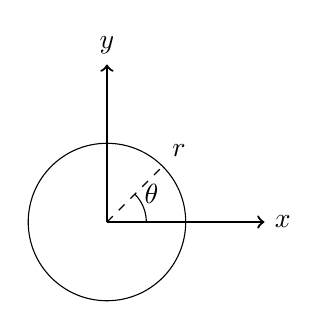
\begin{tikzpicture}
					\draw[thick, ->] (0,0) -- (0,2) node[anchor = south]{$y$};
					\draw[thick, ->] (0,0) -- (2,0) node[anchor = west]{$x$};

					\draw (0,0) circle (1);
					\draw[dashed] (0,0) -- (0.707,0.707) node[anchor = south west]{$r$};
					\draw (0.5,0) arc (0:45:0.5) node[anchor = west]{$\theta$};
				\end{tikzpicture}
			\end{center}
			For a circle, $r = R$
			\begin{align}
				\implies d\vec{\Gamma} = dr\,\hat{r} + r\,d\theta\,\hat{\theta} =  \left(r\,\hat{\theta} + \frac{dr}{d\theta}\,\hat{r}\right)\,d\theta = r\,d\theta\,\hat{\theta}
			\end{align}
			\begin{align}
				\oint_\Gamma \vec{v}\cdot d\vec{\Gamma} &= \int^{\theta=2\pi}_{\theta=0} R^2(-a\sin^2\theta + b\cos^2\theta)\,d\theta = (b-a)\pi R^2
			\end{align}
		\end{solution}
		\subpart Cartesian
		\begin{solution}
			\begin{center}
				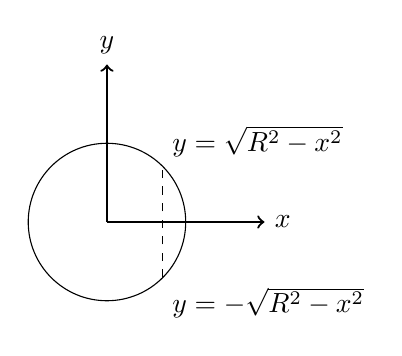
\begin{tikzpicture}
					\draw[thick, ->] (0,0) -- (0,2) node[anchor = south]{$y$};
					\draw[thick, ->] (0,0) -- (2,0) node[anchor = west]{$x$};

					\draw (0,0) circle (1);
					\draw[dashed] (0.707,-0.707) node[anchor = north west]{$y=-\sqrt{R^2-x^2}$} -- (0.707,0.707) node[anchor = south west]{$y=\sqrt{R^2-x^2}$};
				\end{tikzpicture}
			\end{center}
			Let us divide the circle into two parts $y\geq0$ \& $y<0$. For a circle, $y = \pm\sqrt{R^2-x^2}$
			\begin{align}
				\implies d\vec{\Gamma} = dx\,\hat{\imath} + dy\,\hat{\jmath} =  \left(\hat{\imath} + \frac{dy}{dx}\,\hat{\jmath}\right)\,dx = \left(\hat{\imath}\,\mp\,\frac{x}{\sqrt{R^2-x^2}}\,\hat{\jmath}\right)\,dx 
			\end{align}
			\begin{align}
				\oint_{\Gamma} \vec{v}\cdot d\vec{\Gamma} &= \int^{x=-R}_{x=R} (a\sqrt{R^2-x^2}\,\hat{\imath} + bx\,\hat{\jmath})\cdot(\hat{\imath} - \frac{x}{\sqrt{R^2-x^2}}\,\hat{\jmath})\,dx \\
				&+ \int^{x=R}_{x=-R} (-a\sqrt{R^2-x^2}\,\hat{\imath} + bx\,\hat{\jmath})\cdot(\hat{\imath} + \frac{x}{\sqrt{R^2-x^2}}\,\hat{\jmath})\,dx \\
				&= \int^{x=R}_{x=-R} -2a\sqrt{R^2-x^2} + \frac{2bx^2}{\sqrt{R^2-x^2}}\,dx \\
				&= (b-a)\pi R^2
			\end{align}
		\end{solution}
	\end{subparts}

	\part Imagine a right circular cylinder of length $L$ with its axis parallel to the $z$ axis standing on the circle. Use cylindrical co-ordinate system to show that the Stokes theorem is valid over its surface.
	\begin{solution}
		\begin{center}
			\tdplotsetmaincoords{80}{45}
			\begin{tikzpicture}[tdplot_main_coords]
				\draw[thick,->] (0,0,0) -- (3,0,0) node[anchor=north east]{$x$};
				\draw[thick,->] (0,0,0) -- (0,3,0) node[anchor=north west]{$y$};
				\draw[thick,->] (0,0,0) -- (0,0,3) node[anchor=south]{$z$};

				\begin{scope}[canvas is xy plane at z=0]
					\draw (0,0) circle (1);
				\end{scope}

				\begin{scope}[canvas is xy plane at z=1.5]
					\draw (0,0) circle (1);
				\end{scope}

				\draw (0.707,0.707,0) -- (0.707,0.707,1.5);
				\draw (-0.707,-0.707,0) -- (-0.707,-0.707,1.5);

				\draw (-0.707,-0.707,0.75) node[anchor = east]{$L$};

			\end{tikzpicture}
		\end{center}
		According to Stokes theorem,
		\begin{equation}
			\iint_S \nabla\times\vec{v}\cdot\,d\vec{S} = \oint_{\Gamma} \vec{v}\cdot d\vec{\Gamma}
		\end{equation}
		Let us find $\nabla\times\vec{v}$
		\begin{equation}
			\nabla\times\vec{v}
			=
			\left|\begin{matrix}
				\hat{\imath} & \hat{\jmath} & \hat{k} \\
				\frac{\partial}{\partial x} & \frac{\partial}{\partial y} & \frac{\partial}{\partial z} \\
				ay & bx & 0
			\end{matrix}\right|
			= (b-a)\,\hat{k} = (b-a)\,\hat{z}
		\end{equation}
		We need to find $d\vec{S_1}$ of the curved part of the cylinder. We can find it out using parametrization (Ugh! Not MA 105 again!):
		\begin{align}
			\vec{r} &= R\cos\phi\,\hat{\imath} + R\sin\phi\,\hat{\jmath} + z\,\hat{k} \\
			\vec{r}_\phi &= (R\sin\phi\,\hat{\imath} + R\cos\phi\,\hat{\jmath})\,d\phi \\
			\vec{r}_z &= (z\,\hat{k})\,dz \\
			d\vec{S} &= \frac{\vec{r}_\phi\times\vec{r}_z}{|\vec{r}_\phi\times\vec{r}_z|} = (\cos\phi\,\hat{\imath} + \sin\phi\hat{\jmath})\,d\phi\,dz= d\phi\,dz\,\hat{\rho}
		\end{align}
		We also need $d\vec{S_2}$ of the top part of the cylinder. It can similarly be found to be $d\vec{S_2} = \rho\,d\rho\,d\phi\,\hat{z}$
		\begin{align}
			\text{LHS } = \iint_S \nabla\times\vec{v}\cdot\,d\vec{S} &= \int^{\phi=2\pi}_{\phi=0}\int^{z=\frac{L}{2}}_{z=\frac{L}{2}}\cancelto{0}{(b-a)\,\hat{z}\cdot\hat{\rho}\,d\phi\,dz} \\
			&+ \int^{\phi=2\pi}_{\phi=0}\int^{r=R}_{r=0} (b-a)\,\hat{z}\cdot\hat{z}\,\rho\,d\rho\,d\phi \\
			&= (b-a)\pi R^2 = \text{ RHS} \hskip0.4\textwidth\blacksquare
		\end{align}
	\end{solution}
\end{parts}

\question Although the gradient, divergence and curl theorems are the fundamental integral theorems of vector calculus, it is possible to derive a number of corollaries from them. Show that:\label{q:7}
\begin{parts}
	\part \label{eq} $\int_{V}(\nabla T)\,dV=\oint_{S}T\,d\vec{S}$
	[Hint: Let $\vec{v}=\vec{c}\,T$ where $\vec{c}$ is a constant, in the divergence theorem]
	\begin{solution}
		\begin{align}
			\iiint_V \nabla\cdot\vec{v}\,dV &= \oiint_S \vec{v}\cdot d\vec{S} \\
			\implies \iiint_V \nabla\cdot(\vec{c}\,T)\,dV &= \oiint_S (\vec{c}\,T)\cdot d\vec{S} \\
			\implies \cancelto{0}{\iiint_V T\,(\nabla\cdot\vec{c})\,dV} + \vec{c}\cdot\iiint_V (\nabla T)\,dV &= \vec{c}\cdot\oiint_S T\,d\vec{S} \\
			\implies \iiint_V (\nabla T)\,dV &= \oiint_S T\,d\vec{S} \hskip0.3\textwidth\blacksquare
		\end{align}
	\end{solution}

	\part $\int_{V}(\nabla\times\vec{v})\,dV=-\oint_S\vec{v}\times d\vec{S}$ \label{p:7b}
	[Hint: Replace $\vec{v}$ by $\vec{v}\times\vec{c}$, where $\vec{c}$ is a constant in the divergence theorem ]
	\begin{solution}
		\begin{align}
			\iiint_V \nabla\cdot(\vec{v}\times\vec{c})\,dV &= \oiint_S (\vec{v}\times\vec{c})\cdot d\vec{S} \\
			\implies \vec{c}\cdot\iiint_V T\,(\nabla\times\vec{v})\,dV - \cancelto{0}{\iiint_V \vec{v}\cdot(\nabla\times\vec{c})\,dV} &= -\vec{c}\cdot\oiint_S \vec{v}\times d\vec{S} \\
			\implies \iiint_V (\nabla\times\vec{v})\,dV &= -\oiint_S \vec{v}\times d\vec{S} \hskip0.18\textwidth\blacksquare
		\end{align}
	\end{solution}
\end{parts}

\end{questions}
\end{document}